\documentclass{article}
\usepackage{etoolbox}
\usepackage{graphicx}

\ifdef{\myoutput}{}{\def\myoutput{concept}}
\ifdef{\myversion}{}{\def\myversion{1}}

\usepackage[output=\myoutput
,numberofversions=4
,version=\myversion
,seed=4
,randomizequestions=true
,randomizeanswers=true
,writeRfile=true
]{mcexam}

\usepackage[margin=0.95in]{geometry}
\usepackage{multicol}

\usepackage{fancyhdr,lastpage}
\pagestyle{fancy}
\fancyhf{}
\renewcommand{\headrulewidth}{1pt} 
\renewcommand{\footrulewidth}{1pt}
\lfoot{\mctheversion}
\rfoot{Page \thepage\ of \pageref{LastPage}}
\lhead{Quiz 8.3 and 9.2 \mctheversion \\ MAT 2000: Introduction to Statistics}
\rhead{Name Print): \hspace{2.5 in}}

\usepackage{calc}
\renewenvironment{setmcquestion}
{\begin{minipage}[t]{\linewidth-\labelwidth}}
	{\end{minipage}\par}
	
\renewenvironment{setmcquestioninstruction}
{\begin{minipage}{\textwidth}}
	{\end{minipage}}
	
\renewenvironment{setmcanswers}{}{}
\setlist[setmcquestions]{label=\mcquestionlabelfmt{*}.
	,ref=\mcquestionlabelfmt{*}
	,itemsep=0.5\baselineskip
	,topsep=1\baselineskip
}

\renewcommand\mcversionlabelfmt[1]{\arabic{#1}}

%copy-pasting from MS Word, use regex to find [\*]*[a-d]\. and replace with \answer 

\raggedbottom

\begin{document}
	Circle the correct answer for each question.  If you're unsure, you can write numbers 1, 2, 3, etc. next to the choices to get partial credit.  Questions refer to the nonindented paragraph above unless otherwise stated.\\[.5cm]
	
	\begin{mcquestions}
		\begin{mcquestioninstruction}
			As part of a study, twenty students rated their own attractiveness on a scale from 1 – 10, and had a picture taken.  In the second part of the study, a group of 79 college student volunteers (not part of the original group of 20) rated the attractiveness of each of the 20 students in the pictures on a scale of 1 – 10.  Researchers averaged the attractiveness rating of the 79 "raters" (referred to as the societal rating) to compare to the self-rating to determine whether or not college students are accurate in their self-perceptions. Summary statistics are presented in the following table. The average difference in attractiveness ratings (self – societal) in the sample was 1.066 with a standard deviation of 1.507. A dotplot of these differences follows.
			\begin{center}
				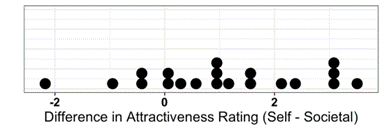
\includegraphics[width=0.8\textwidth]{self-societal.png}
			\end{center}
			Use this scenario to answer questions \ref{self-societal-1}, \ref{self-societal-2}, and \ref{self-societal-3}.
		\end{mcquestioninstruction}
		\question Would a theoretical approach be valid to analyze these data? \label{self-societal-1}
		\begin{mcanswerslist}
			\answer Yes, since the sample size of 79 is at least 20, and the distribution of differences is not strongly skewed.
			\answer Yes, since the sample size of 40 is at least 20, and the distribution of differences is not strongly skewed.
			\answer[correct] Yes, since the sample size of 20 is at least 20, and the distribution of differences is not strongly skewed.
			\answer No, a theoretical approach would not be valid because the sample size is too small.
		\end{mcanswerslist}
		
		\question[follow] Calculate the standard error of the sample mean difference in attractiveness ratings (self $–$ societal).\label{self-societal-2}
		\begin{mcanswerslist}
			\answer 1.066
			\answer 3.163
			\answer 1.507
			\answer[correct] 0.337
		\end{mcanswerslist}
		
		\question[follow] Based on the standardized statistic for this scenario, what is the conclusion? \label{self-societal-3}
		\begin{mcanswerslist}
			\answer[correct] Strong evidence exists that students similar to those in the study are \textit{not} accurate in their self-perception of attractiveness, on average.
			\answer Strong evidence exists that students similar to those in the study are accurate in their self-perception of attractiveness, on average.
			\answer No evidence exists that students similar to those in the study are accurate in their self-perception of attractiveness, on average.
			\answer No evidence exists that students similar to those in the study are not accurate in their self-perception of attractiveness, on average.
		\end{mcanswerslist}
		
		\question Researchers randomly selected 36 children who had been identified as gifted from a large city. The IQ of each child and the IQ of the child's mother were measured. A statistical analysis will be performed to determine if IQs of gifted children tend to be higher than their mothers' IQ on average. The mean difference in IQ (child – mother) was 3.22 points, with a standard deviation of 7.41 points.
		
		The p-value for these data is 0.0067. Would the results of this study be considered statistically significant at the 5\% significance level?  Select one. 
		\begin{mcanswerslist}
			\answer Yes, because random sampling was used.
			\answer No, because groups were not randomly assigned.
			\answer[correct] Yes, because the p-value is less than 0.05.
			\answer No, because the validity conditions were not met.
		\end{mcanswerslist}
		
		
		\question Suppose the chi-square statistic for a test was 6.991. If instead, the chi-square statistic had been 5.332, would the p-value be smaller, larger, or remain the same?
		\begin{mcanswerslist}
			\answer Smaller
			\answer[correct] Larger
			\answer Remain the same
			\answer Cannot be determined
		\end{mcanswerslist}
		
		\begin{mcquestioninstruction}
			Grace College student researchers want to determine if students yawning (when being yawned at) is associated with the time of day (morning, afternoon, and evening). The students found the following results from yawning in front of people around campus:
			\begin{itemize}
				\item Morning: 25 of the 39 people yawned back
				\item Afternoon: 15 of the 38 people yawned back
				\item Evening: 29 of the 44 people yawned back
			\end{itemize}
			Use this scenario to answer questions \ref{yawn-1} and \ref{yawn-2}.
		\end{mcquestioninstruction}
		\question When this test is run, a p-value of 0.03 is found. What would be an appropriate conclusion? \label{yawn-1}
		\begin{mcanswerslist}
			\answer Strong evidence exists that the probability a person yawns is different between all three times of day: morning, afternoon, and evening.
			\answer[correct] Strong evidence exists of an association between time of day and whether a person yawns.
			\answer Strong evidence of no association between time of day and whether a person yawns.
			\answer Strong evidence does not exist of an association between time of day and whether a person yawns.
		\end{mcanswerslist}
		
		\question[follow] After a chi-square test, follow-up confidence intervals for all pairwise differences in proportions are found as follows: \label{yawn-2}
		\begin{itemize}
			\item 0.0299 to 0.4627:  Morning – Afternoon
			\item -0.2237 to 0.1876:  Morning – Evening
			\item -0.4736 to -0.0551:  Afternoon – Evening
		\end{itemize}
		Based off of these intervals, which of the following conclusions are correct?
		\begin{mcanswerslist}
			\answer The probability of yawning in the morning differs significantly from the probability of yawning in the evening.
			\answer[correct] The probability of yawning in the morning differs significantly from the probability of yawning the afternoon.
			\answer The probability of yawning in the afternoon does not differ significantly from the probability of yawning in the evening.
			\answer The probability of yawning in the morning does not differ significantly from the probability of yawning in the afternoon.
		\end{mcanswerslist}
		
		%COMMENTED OUT:
		%I'm not sure I covered this enough:
		%\question Why do we do overall tests when comparing multiple proportions and not just do the follow-up confidence intervals?
		%\begin{mcanswerslist}
		%	\answer[correct] Doing an overall test will more likely lead to significant results than just doing the follow-up confidence intervals.
		%	\answer Doing an overall test allows us to see exactly which group is significantly different from which other groups.
		%	\answer Doing an overall test allows us to quickly get our results, while the follow-up confidence intervals are very time-consuming.
		%	\answer Doing an overall test allows us to keep the probability of a type I error at 5\% or whatever significance level we would like.
		%\end{mcanswerslist}
		
		
		\question Can telling a joke affect whether or not a customer in a coffee bar leaves a tip for the waiter? A study investigated this question at a coffee bar in France. The waiter randomly assigned coffee-ordering customers into three groups: one received a card telling a joke with their bill, another group received a card containing an advertisement for a local restaurant, and the third received no card. The results are shown below.
		\begin{center}
			\begin{tabular}{| l | l | l | l | l |}
				\hline
				& \textbf{Joke Card} & \textbf{Ad Card} & \textbf{No Card} & \textbf{Total} \\
				\hline
				\textbf{Left Tip} & 32 & 16 & 24 & 72 \\
				\hline
				\textbf{No Tip} & 48 & 64 & 56 & 168 \\
				\hline
				\textbf{Total} & 80 & 80 & 80 & 240 \\
				\hline
			\end{tabular}
		\end{center}
		Are validity conditions met to conduct a chi-square test of association?
		\begin{mcanswerslist}
			\answer Yes, since 80 is larger than 20.
			\answer Yes, since 240 is larger than 20.
			\answer[correct] Yes, since each cell in the table has at least 10 observations.
			\answer No, the sample is not a random sample of customers.
		\end{mcanswerslist}
		
		
	\end{mcquestions}
\end{document}